\documentclass[12pt]{article}

% Codificación y lenguaje
\usepackage[utf8]{inputenc}
\usepackage[T1]{fontenc}
\usepackage[spanish]{babel}
\usepackage{newtxtext,newtxmath} % Fuente similar a Times New Roman




% Citas bibliograficas
\usepackage[backend=biber,style=ieee]{biblatex}
\addbibresource{bibliografia.bib}
\usepackage{hyperref}
\usepackage{csquotes}


% Márgenes
\usepackage[a4paper, left=2.5cm, right=2.5cm, top=2cm, bottom=2cm]{geometry}

% Gráficos, flotantes y código
\usepackage{graphicx}
\usepackage{float}
\usepackage{listings}
\usepackage{xcolor}
\usepackage{tikz}
\usepackage{url}

% Encabezados y pies de página
\usepackage{fancyhdr}
\pagestyle{fancy}
\fancyhf{}
\lhead{Estándar CubeSat - PC104}
\rhead{UNC - PPS - Campos Mariano}
\cfoot{\thepage}

% Estilo para código Matlab
\definecolor{codegreen}{rgb}{0,0.6,0}
\definecolor{codegray}{rgb}{0.5,0.5,0.5}
\definecolor{codepurple}{rgb}{0.58,0,0.82}
\definecolor{backcolour}{rgb}{0.95,0.95,0.92}

\lstdefinestyle{mystyle}{
	language=Matlab,
	backgroundcolor=\color{white}, 
	basicstyle=\sffamily\footnotesize,
	keywordstyle=\color[HTML]{0072BD}\bfseries,
	commentstyle=\color[HTML]{008000}\itshape,
	stringstyle=\color[HTML]{A2142F},
	numberstyle=\tiny\color{gray},
	numbers=left,
	numbersep=3pt,
	frame=single,
	rulecolor=\color{black!50},
	breaklines=true,
	tabsize=2,
	showspaces=false,
	showstringspaces=false,
}

% Título y autores
\title{
	
\includegraphics[width=0.45\textwidth]{unc.png} \\[2cm] % Logo
	\textbf{Practicas profesionales supervisadas: Investigación estándar CubeSat - PC104}
}

\author{
	Profesores: \\ Esp. Ing Carlos R.Leguizamon \\ Ing. Oscar Vanella \\ Ing. Conrado J.Rodriguez
	\\
	Alumno: \\ Campos Mariano
}

\date{Mayo de 2025} % Fecha del trabajo

\begin{document}
	
	\maketitle
	
	\begin{abstract}
		En el presente informe se recopila, organiza y clasifica toda la información referida a los estándares CubeSat y PC-104 con el objetivo de obtener las restricciones de diseño para la fabricación de un transponder. La investigación forma parte del paso previo a la realización de la placa, dado que permite identificar los parámetros mecánicos, eléctricos y de integración que deben cumplirse para garantizar la compatibilidad del sistema dentro de un nanosatélite.
		
		 
	\end{abstract}\newpage
	
	\newpage
	
	\tableofcontents \newpage
	
	\section{Introducción}
		\subsection{Contexto}
		Según el articulo publicado en la universidad politécnica de California (Cal Poly) \cite{CalPoly2023} desde finales de los años 90, los nanosatélites tipo CubeSat han experimentado un crecimiento exponencial impulsado por su bajo costo, construcción rápida y elevada accesibilidad académica y comercial. Este éxito se remonta a 1999, cuando los profesores Jordi Puig-Suari de Cal Poly y Bob Twiggs del Space Systems Development Laboratory de Stanford definieron la especificación del CubeSat como una herramienta educativa para que estudiantes pudieran diseñar, ensamblar y operar satélites funcionales dentro de los límites temporales y financieros de su formación. El diseño estándar consiste en unidades cúbicas de 10 cm por lado (1U) típicamente de 1 kg hasta unos 2 kg, y puede escalarse a configuraciones de 2U, 3U, 6U hasta 12U.
		
		\begin{figure}[h!]
			\centering
			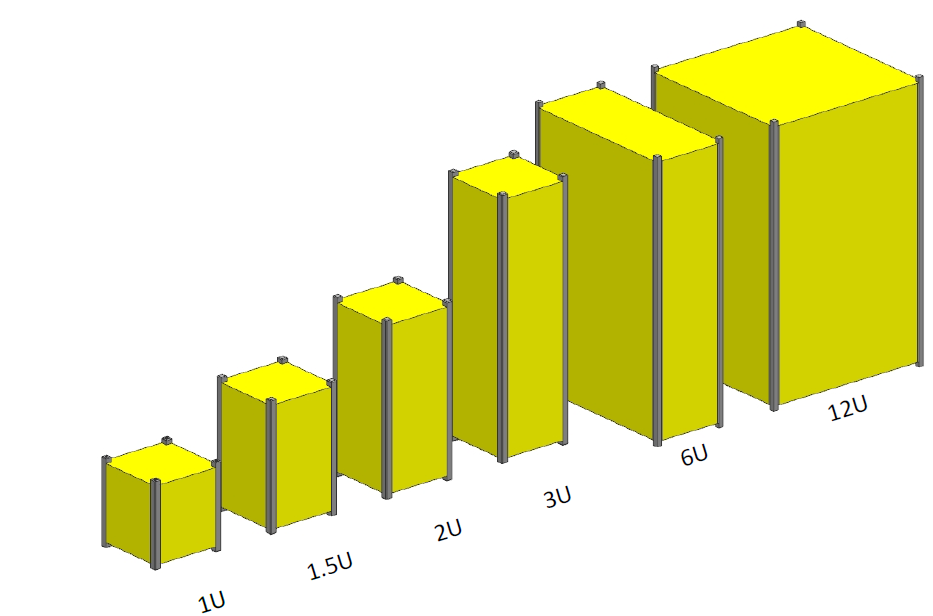
\includegraphics[width=0.7\linewidth]{imagenes/size_cubesat}
			\caption[Unidades cubicas (Fuente: CubeSat Design Specification Rev. 14.1)]{Unidades cubicas (Fuente: CubeSat Design Specification Rev. 14.1)}
			\label{fig:sizecubesat}
		\end{figure}
		
		
		El despliegue del primer CubeSat en órbita ocurrió en junio de 2003, mediante el cohete ruso Dnepr desde Kazajistán, marcando un hito en misiones espaciales universitarias. Desde entonces, el número de CubeSats lanzados ha superado ampliamente los 1660 a inicios de 2022, con más de 700 misiones planificadas solo ese año, incluyendo un número significativo de proyectos de compañías privadas. Esta proliferación refleja una transición significativa: hasta 2013, la mayoría de los CubeSats eran desarrollados por instituciones educativas, pero a partir de entonces más del 50 \% de los lanzamientos corresponden a iniciativas comerciales. Esta evolución evidencia cómo el estándar CubeSat, nacido en el ámbito académico, ha trascendido hacia aplicaciones científicas, tecnológicas, de observación terrestre y comunicación, incluso convirtiéndose en la primera plataforma satelital para muchos países que antes no tenían experiencia espacial. Según palabras de Ryan Nugent, director del Laboratorio CubeSat de Cal Poly:
		 
		\begin{quote}
			``No solo miles de estudiantes de todo el mundo han podido lanzar un satélite, 
			sino que se ha convertido en una industria de mil millones de dólares y ha 
			desempeñado un papel importante en generar un entusiasmo renovado por el 
			espacio que no existía desde el alunizaje''.
		\end{quote}\newpage
		
		En este contexto, el transponder resulta una pieza fundamental dentro de la arquitectura del satélite, encargado de recibir y retransmitir señales de manera confiable. Sin embargo, su diseño no puede desarrollarse aisladamente: debe armonizarse con los estándares de tamaño, masa, energía, etc impuestos por el CubeSat, ademas de los requerimientos funcionales del propio transponder como lo pueden ser ancho de banda, número de canales, potencia, control de ganancia, relación señal-ruido, etc. La arquitectura electrónica modular, en particular la basada en PC104, ha sido ampliamente adoptada en diseño de subsistemas satelitales. Este estándar define un factor de forma compacto y permite el apilamiento de placas, con conectores robustos adecuados para entornos de vibración y espacio.
		
		Por estas razones, comprender a fondo el entorno normativo en el que se integran los CubeSats es un requisito esencial antes de avanzar en el diseño de un transponder. Esto garantiza su viabilidad técnica, compatibilidad con otros módulos, alineación con prácticas internacionales y, en última instancia, su potencial para ser parte de una misión espacial real.
		
		\subsection{Objetivo del informe}
		El objetivo principal de este informe es recopilar, organizar y analizar la información disponible sobre los estándares CubeSat y PC104, con el fin de determinar las restricciones de diseño aplicables a la fabricación de un transponder para su integración en un nanosatélite. La investigación busca establecer un marco técnico y normativo que permita garantizar que el transponder cumpla con los requerimientos mecánicos, eléctricos y de comunicación necesarios para operar de manera confiable dentro de la plataforma CubeSat.
		
		En particular, se pretende identificar los parámetros críticos como dimensiones físicas, masa, consumo energético, interfaces de conexión y compatibilidad electromagnética, así como comprender cómo la arquitectura modular basada en PC104 facilita la integración con otros subsistemas del satélite (OBC, EPS, sistemas de telemetría). Este análisis constituye un paso previo al diseño de la placa, ya que asegura que las decisiones de ingeniería estén alineadas con estándares internacionales, reduciendo riesgos de incompatibilidad, fallas técnicas y sobrecostos en etapas posteriores del proyecto.
		
		\subsection{Alcance de la investigación}
		La investigación abarca principalmente los siguientes aspectos:
		\begin{itemize}
			\item Restricciones mecánicas: dimensiones físicas, peso máximo permitido, tolerancias estructurales, materiales,etc.
			\item Restricciones eléctricas y energéticas: consumo de energía, voltajes  y frecuencias de operación, compatibilidad con la fuente de alimentación del satélite, etc.
			\item Interfaces y conectividad: forma de apilamiento y conexiones definidas por el estándar PC104, incluyendo compatibilidad con otros subsistemas del CubeSat, como el OBC (On-Board Computer), EPS (Electrical Power System) y sistemas de telemetría.
			\item Otras consideraciones: Cuestiones como ensayos a los que debe ser sometido, vibraciones, compatibilidad electromagnética, etc. Así como también requerimientos legales, permisos necesarios para poder operar sin restricciones.
		\end{itemize}
		
		Quedan fuera del alcance del presente informe aspectos relacionados con el diseño detallado de circuitos, programación de firmware, pruebas de laboratorio o simulaciones de RF, los cuales serán abordados en etapas posteriores del proyecto.
		
	\section{Desarrollo}
	\subsection{Especificaciones CubeSat}
	El CubeSat Design Specification (CDS) es el documento oficial de Cal Poly \cite{CDS2022} (versión vigente: Rev. 14.1, febrero 2022) que establece el conjunto de reglas que garantizan que cualquier CubeSat pueda ser lanzado de manera segura y compatible en un cohete comercial.
	Los lanzadores son los vehículos espaciales (cohetes) que transportan los CubeSats al espacio. La gran mayoría de CubeSats no viajan como carga primaria, sino como carga secundaria (piggyback) junto con satélites grandes.
	Para que esto sea posible, los CubeSats deben cumplir estrictamente con las dimensiones, masa y restricciones mecánicas/eléctricas definidas en el estándar, de modo que puedan ser integrados en un dispensador (el más famoso es el Poly Picosatellite Orbital Deployer – P-POD).El dispensador se instala en el lanzador y se encarga de guiar, contener y liberar a los CubeSats en la órbita asignada.
	
	Es importante discernir que, en el documento se utiliza tres \textbf{"Términos operativos"} diferentes a la hora de enumerar las distintas especificaciones:
	
	\begin{itemize}
		\item \textbf{"Deberá"}: se utiliza para indicar requisitos que deben cumplirse y que requieren verificación formal.
		
		\item \textbf{"Debería"}: se utiliza para indicar una recomendación firme o una sugerencia para facilitar la verificación formal de otro requisito.En muchos casos, el incumplimiento limitará oportunidades de lanzamiento.
		
		\item \textbf{"Será"}: sirven para indicar eventos para los que los desarrolladores de naves espaciales deben estar preparados.
		
		\item \textbf{"Nota"}: se utiliza para indicar una recomendación o consejo destinado a ayudar al desarrollador del CubeSat.
	\end{itemize}
	
	\subsubsection{Especificaciones generales}
	
	\begin{enumerate}
		\item Todas las piezas deberán permanecer unidas a los CubeSats durante el lanzamiento, la eyección y el funcionamiento.
		
		\item Los artículos pirotécnicos deberán cumplir con AFSPCMAN 91-710, (Volumen 3). \cite{AFSPCMAN91710}
		
		\item Todos los sistemas de propulsión deberán diseñarse, integrarse y probarse de acuerdo con AFSPCMAN 91-710 (Volumen 3).
		
		\item Los sistemas de propulsión deberán tener al menos tres inhibidores de activación.
		
		\item Nota: Se recomienda tener en cuenta los requisitos de la Administración Federal de Aviación (FAA) \cite{FAA2025Lithium} para las baterías transportadas por pasajeros de aerolíneas. La capacidad máxima permitida para baterías de iones de litio de tamaño estándar en el equipaje de mano es de 100 Wh por batería. 
		
		\item Los materiales peligrosos del CubeSat deberán cumplir con AFSPCMAN 91-710, (Volumen 3).
		
		\item Los materiales de los CubeSats deberán cumplir con los criterios de baja desgasificación, según se define en los dos apartados siguientes, para evitar la contaminación de otras naves espaciales durante la integración, las pruebas y el lanzamiento. Puede consultar una lista de materiales de baja desgasificación aprobados por la NASA \cite{NASA2025OutgassingDB}
		
		\subitem $\bullet$ Los materiales de los CubeSats deberán tener una pérdida de masa total (TML) inferior o igual al 1,0 \%.
		\subitem $\bullet$ Los materiales de los CubeSats deberán tener un material condensable volátil recolectado (CVCM) inferior o igual al 0,1 \%.
		
		\item El campo magnético de cualquier imán pasivo se limitará a 0,5 Gauss por encima del campo magnético de la Tierra, fuera de la envoltura estática del CubeSat.Evita riesgos de interferencia electromagnética, problemas en el dispensador y contaminación de mediciones científicas.
		
		\item El CubeSat deberá diseñarse para permitir ventilación durante el ascenso, de manera que la relación volumen ventilable/área de ventilación sea menor a 50,8 metros.Cuando el cohete asciende desde la Tierra hacia el espacio, la presión atmosférica disminuye rápidamente, por eso se exige que el satélite tenga orificios de ventilación “vent holes” que permitan al aire salir controladamente durante el ascenso, esto garantiza que el aire atrapado pueda evacuar lo suficientemente rápido para que no se acumulen presiones internas peligrosas.
		
	\end{enumerate}
	
	\subsubsection{Especificaciones mecánicas}
	Los planos donde se especifican las dimensiones y características del CubeSat se pueden encontrar en la siguiente sección \cite{CDSDrawings2022}
	
	\begin{enumerate}
		\item Nota: El Procedimiento de Inspección y Comprobación de Ajuste (CIFP) \cite{CIFP2020} del CubeSat puede utilizarse para verificar que el CubeSat cumple con los requisitos dimensionales especificados.
		
		\item El origen del sistema de coordenadas del CubeSat se encuentra en el centro geométrico del CubeSat.
		
		\begin{figure}[h!]
			\centering
			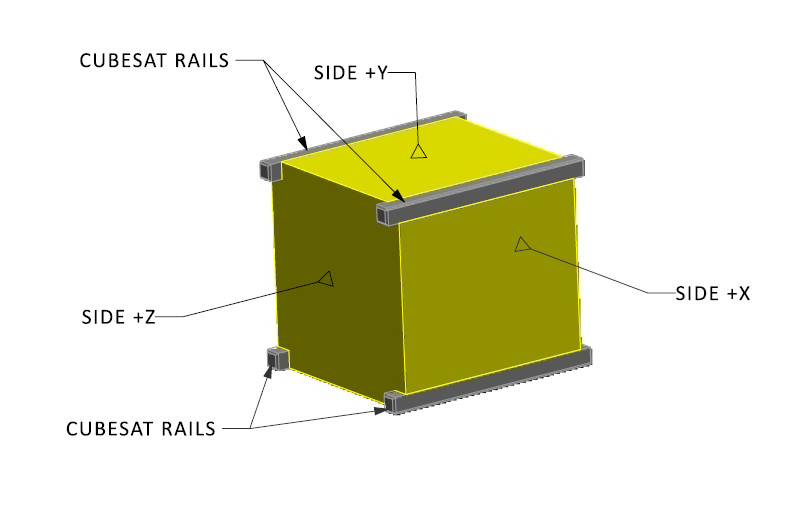
\includegraphics[width=0.7\linewidth]{imagenes/xyz_cubesat}
			\caption[Sistema de referencias CubeSat ejes coordenados ()]{Sistema de referencias CubeSat ejes coordenados (Fuente: CDSDrawings2022)}
			\label{fig:xyzcubesat}
		\end{figure}
		
		
		\item La configuración y las dimensiones físicas del CubeSat deberán cumplir con la sección correspondiente especificado en el plano.
		
		\item Nota: La dimensión de la longitud del separador de $5.0$ a $7.0$ mm con tolerancia de $0.1$ mm en la cara $\pm$ Z, especificada en los planos, existe para evitar interferencia con posibles CubeSats vecinos y con las interfaces del dispensador.Las caras $\pm$ Z son las que se orientan en el eje de eyección dentro del P-POD, por tanto, son las más críticas para asegurar que nada sobresalga más allá de lo permitido.
		
		\begin{figure}[h!]
			\centering
			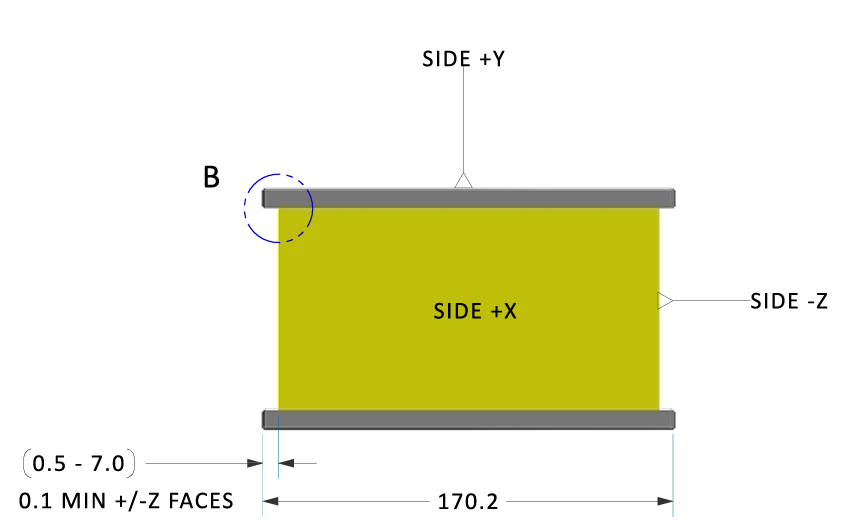
\includegraphics[width=0.7\linewidth]{imagenes/z_face_cubesat}
			\caption[Tolerancias del separador  (Fuente: CDSDrawings2022)]{Tolerancias del separador  (Fuente: CDSDrawings2022)}
			\label{fig:zfacecubesat}
		\end{figure}
		
		
		
		\item Nota: Puede haber volumen adicional disponible para CubeSats de 3U, 6U y 12U. Este volumen adicional a veces se denomina volumen de la "lata de atún". La disponibilidad y las dimensiones del volumen dependen del dispensador. (Figura 4 y 5)
		
		\begin{figure}[h!]
			\centering
			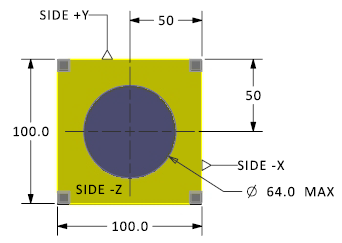
\includegraphics[width=0.4\linewidth]{imagenes/extra_vol_2_cubesat}
			\caption[Volumen extra configuraciones para configuración 1U (Fuente: CDSDrawings2022)]{Volumen extra configuraciones para configuración 1U (Fuente: CDSDrawings2022)}
			\label{fig:extravol2cubesat}
		\end{figure}
		
		\begin{figure}[h!]
			\centering
			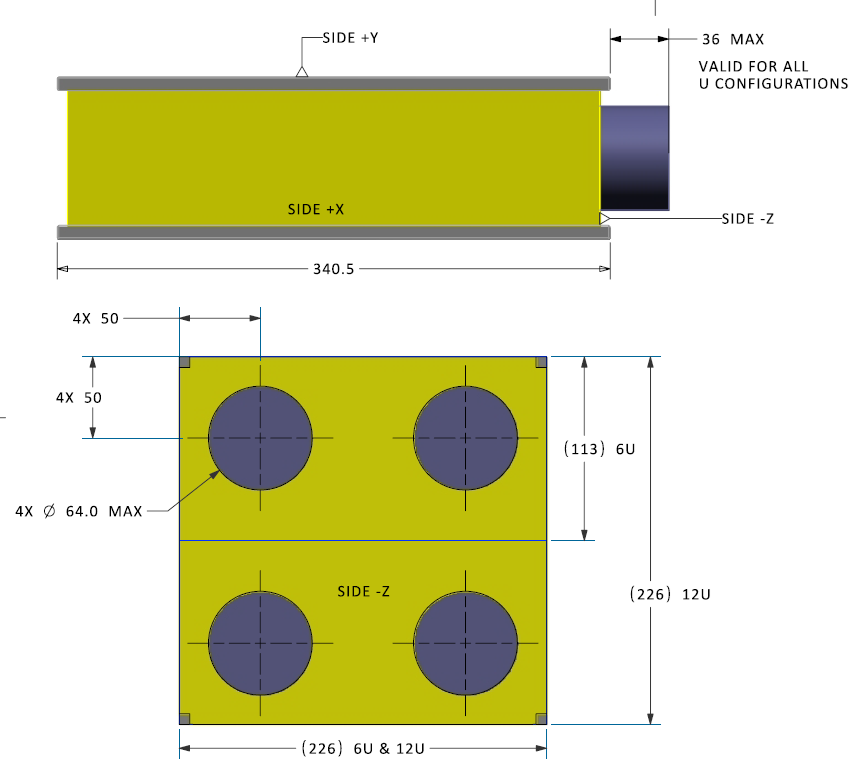
\includegraphics[width=0.7\linewidth]{imagenes/extra_vol_cubesat}
			\caption[Volumen extra configuraciones para configuración 6U y 12U (Fuente: CDSDrawings2022)]{Volumen extra configuraciones para configuración 6U y 12U (Fuente: CDSDrawings2022)}
			\label{fig:extravolcubesat}
		\end{figure}\newpage
		
		\item La cara –Z del CubeSat se insertará primero en el dispensador.
		
		\item Ningún componente de los lados sombreados en amarillo (ver dibujos del CDS \cite{CDSDrawings2022}) no debe sobresalir más de 6,5 mm normal a la superficie desde el plano del riel.
		
		\item Nota: Consulte el CIFP (CubeSat Inspection and Fit-check Procedure) \cite{CIFP2020} para conocer la técnica de medición de protuberancia recomendada. Este consiste en un procedimiento oficial para verificar que un CubeSat cumple con las especificaciones mecánicas establecidas en el CubeSat Design Specification (CDS).
		
		\item Los elementos desplegables (antenas, paneles solares, booms, etc.) deberán estar asegurados por el propio CubeSat, no por el dispensador. Este requisito proviene de las exigencias de la mayoría de los proveedores de lanzamiento. La norma exige que sea el propio CubeSat quien asegure esos elementos, nunca el dispensador, porque este solo debe actuar como contenedor y no como parte activa del mecanismo de despliegue.
		
		\item Los rieles deberán tener un ancho mínimo de 8,5 mm medido desde el borde del riel hasta la primera protuberancia en cada cara. (Figura 6)
		
		\begin{figure}[h!]
			\centering
			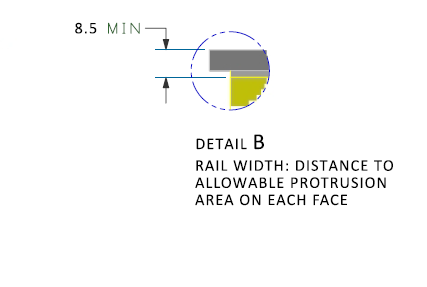
\includegraphics[width=0.45\linewidth]{imagenes/rail_8.5_cubesat}
			\caption[Ancho mínimo del riel hasta la primera protuberancia (Fuente: CDSDrawings2022)]{Ancho mínimo del riel hasta la primera protuberancia (Fuente: CDSDrawings2022)}
			\label{fig:rail8}
		\end{figure}
	
		\item Los rieles deben tener una rugosidad superficial menor a 1,6 um.
		
		\item Los bordes de los rieles deben redondearse con un radio de al menos 1 mm.
		
		\item Los extremos de los rieles en la cara  $\pm$ Z deberán tener una superficie mínima de 6,5 mm x 6,5 mm de área de contacto con los rieles del CubeSat vecinos. Si el CubeSat no comparte el dispensador con otra nave espacial, el proveedor de lanzamiento puede optar por no aplicar este requisito de superficie.
		
		\item Al menos el 75$\%$ del riel debe estar en contacto con los rieles del dispensador. El 25$\%$ restante del riel puede estar empotrado (retraído).
		
		\item El Cuadro 1 muestra la masa máxima típica para cada configuración en U. Las masas aceptables pueden variar según las capacidades del dispensador. Las masas superiores a la presentada en la Cuadro 1 pueden evaluarse misión por misión.
		
		\begin{table}[h!]
			\centering
			\renewcommand{\arraystretch}{1}
			\begin{tabular}{|c|c|}
				\hline
				Configuración U & Masa [Kg]   \\
				\hline
				1U   & 2.00  \\ \hline
				1.5U & 3.00  \\ \hline
				2U   & 4.00  \\ \hline
				3U   & 6.00  \\ \hline
				6U   & 12.00 \\ \hline
				12U  & 24.00 \\ \hline
			\end{tabular}
			\caption{Masa máxima permitida según configuración CubeSat (Fuente: CDS Rev. 14.1).}
			\label{tab:cubesat_mass}
		\end{table}
		
		\item El centro de gravedad del CubeSat deberá estar dentro de los rangos especificados en el Cuadro 2.
		
		\begin{table}[h!]
			\centering
			\renewcommand{\arraystretch}{1} % más espacio entre renglones
			\begin{tabular}{|c|c|c|c|}
				\hline
				Configuración U & Eje X & Eje Y & Eje Z \\
				\hline
				1U   & +2 cm / -2 cm & +2 cm / -2 cm & +2 cm / -2 cm \\ \hline
				1.5U & +2 cm / -2 cm & +2 cm / -2 cm & +3 cm / -3 cm \\ \hline
				2U   & +2 cm / -2 cm & +2 cm / -2 cm & +4.5 cm / -4.5 cm \\ \hline
				3U   & +2 cm / -2 cm & +2 cm / -2 cm & +7 cm / -7 cm \\ \hline
				6U   & +4.5 cm / -4.5 cm & +2 cm / -2 cm & +7 cm / -7 cm \\ \hline
				12U  & +4.5 cm / -4.5 cm & +4.5 cm / -4.5 cm & +7 cm / -7 cm \\
				\hline
			\end{tabular}
			\caption{Rangos aceptables de ubicación del centro de gravedad medidos desde el centro geométrico en cada eje principal (Fuente: CDS Rev. 14.1).}
			\label{tab:centro_gravedad}
		\end{table}
		
		\item La estructura del CubeSat debe estar hecha de aleación de aluminio. Normalmente, se utiliza aluminio 7075, 6061, 6082, 5005 o 5052 tanto para la estructura principal del CubeSat como para los rieles. Si se utilizan materiales distintos del aluminio, el desarrollador del CubeSat debe contactar al proveedor de lanzamiento o al fabricante del dispensador.
		
		\item Cualquier superficie externa de aluminio del CubeSat, como los rieles y separadores que estén en contacto con los rieles del dispensador, deberá estar anodizada en duro (Es un proceso electroquímico que recubre el aluminio con una capa de óxido muy dura y aislante) para prevenir cualquier soldadura en frío dentro del dispensador. En el vacío, dos superficies metálicas limpias y sin recubrimiento pueden fusionarse espontáneamente al entrar en contacto bajo presión, aunque estén a temperatura ambiente.
		
		\item Si un CubeSat comparte un dispensador con otro(s) CubeSat(s), cada CubeSat deberá emplear un mecanismo que favorezca la separación respecto de los CubeSats vecinos dentro del dispensador. Cualquier mecanismo que proporcione separación es aceptable, resortes, imanes, etc. La creencia común con los resortes de separación es que “cuanto más fuerte”, mejor. Esto no siempre es así. Los resortes de separación más fuertes pueden superar la fuerza del resorte de despliegue del dispensador CubeSat durante la expulsión y producir características de separación impredecibles, lo que podría volver a contactar con los CubeSats vecinos. Por otro lado, los resortes de menor fuerza podrían no tener la energía suficiente para separar los CubeSats en la medida necesaria. La recomendación general es seleccionar un resorte de separación con una fuerza máxima inferior a 6,7 N pero con una longitud de carrera superior a 2,5 mm.
		
		\item El mecanismo de separación no deberá extenderse más allá del nivel del separador (standoff) en configuración almacenada (stowed configuration). Los standoffs son pequeños separadores mecánicos que definen la superficie máxima permitida hacia afuera de la estructura del CubeSat, es como un “tope” dimensional para que nada sobresalga más allá de lo permitido en las caras ±Z o en los rieles.
		
		\item Nota: La ubicación más común del mecanismo de separación del CubeSat es centrada en el extremo de los dos standoffs de la cara –Z del CubeSat como se muestra en la figura 7.
		
		\item Nota: No se requiere un mecanismo de separación para CubeSats que no compartan un dispensador con otro(s) CubeSat(s).
		
		\begin{figure}[h!]
			\centering
			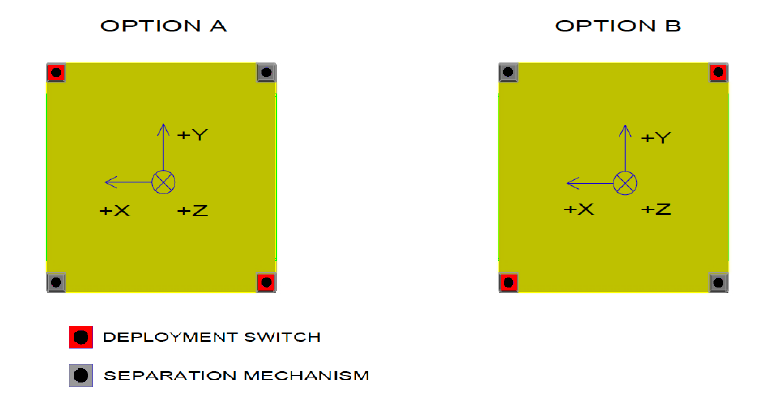
\includegraphics[width=0.7\linewidth]{imagenes/separation_cubesat}
			\caption[Mecanismos de separación cara -Z (Fuente: CDSDrawings2022)]{Mecanismos de separación cara Z (Fuente: CDSDrawings2022)}
			\label{fig:separationcubesat}
		\end{figure}
		
	\end{enumerate}
	
	\subsubsection{Especificaciones eléctricas}
	Los sistemas electrónicos se diseñarán con las siguientes características de seguridad.
	
	
	\begin{enumerate}
		\item Para evitar que el CubeSat active cualquier función que requiera energía, el sistema de potencia del CubeSat deberá permanecer en estado apagado desde el momento de la entrega al vehículo de lanzamiento hasta el despliegue en órbita.
		
		\item Nota: Las funciones alimentadas del CubeSat incluyen la variedad de subsistemas como C\&DH, comunicación por RF,ADC, activación de mecanismos desplegables, etc. Los sistemas de potencia del CubeSat incluyen todos los conjuntos de baterías y celdas solares.
		
		\item Los CubeSats deberán incorporar protección de circuito de batería para la carga/descarga con el fin de evitar condiciones de celdas desbalanceadas. Se requerirá documentación adicional del fabricante y/o ensayos para celdas modificadas, personalizadas o que no estén certificadas bajo UL (Underwriters Laboratories), norma de seguridad internacional.
		
		\item El CubeSat deberá tener, como mínimo, un interruptor de despliegue (deployment switch), el cual se acciona mientras está integrado en el dispensador. Este mantiene el satélite apagado mientras esté dentro del dispensador. Solo al ser liberado en órbita este interruptor se desactiva, permitiendo encender el sistema de manera segura.
		
		\item En el estado activado, el interruptor de despliegue del CubeSat desconectará eléctricamente el sistema de energía de las funciones alimentadas.
		
		\item El interruptor de despliegue deberá estar en estado activado en todo momento mientras esté integrado en el dispensador.
		
		\item En estado activado, el interruptor de despliegue del CubeSat debe estar al nivel o por debajo de cualquier superficie externa que interactúe con el dispensador o el CubeSat adyacente. Esto garantiza que el interruptor no dañe ni interfiera con la superficie de contacto.
		
		\item Si el interruptor de despliegue del CubeSat cambia del estado activado al estado anterior al lanzamiento, el satélite se restablecerá a un estado previo al lanzamiento, lo que incluye el reinicio de la transmisión y los temporizadores.
		
		\item Se podrán permitir los relojes de tiempo real (RTC) si cumplen los requisitos:
		
		\subitem $\bullet$ Los circuitos RTC deberán estar aislados del sistema de alimentación principal.
		\subitem $\bullet$ Las frecuencias RTC deberán ser inferiores a 320 kHz
		\subitem $\bullet$ Los circuitos RTC deberán tener una corriente limitada a menos de 10 mA.
		
		\item El pin RBF (Remove Before Flight) y todos los conectores umbilicales del CubeSat deberán estar dentro de las ubicaciones de puertos de acceso designados, si estos están disponibles en el dispensador del CubeSat.
		
		\item Nota: Algunos dispensadores no tienen puertos de acceso, por lo que es necesario retirar el RBF antes de insertarlo en el dispensador. Se recomienda que el desarrollador del CubeSat tenga en cuenta esta posibilidad al diseñar la secuencia de encendido y arranque.
		
		\item El CubeSat incluirá un pin RBF, que corta toda la energía al satélite una vez que se inserta en él.
		
		\item El pin RBF deberá retirarse del CubeSat antes de la integración en el dispensador, si este no dispone de puertos de acceso.
		
		\item El CubeSat deberá tener al menos tres inhibidores de RF independientes para impedir la transmisión de RF involuntaria.
		
		\item Nota: Un inhibidor es un dispositivo físico entre una fuente de energía y un peligro.
		
		\item Nota: Un temporizador no se considera un inhibidor independiente.
		
		\item Nota: Algunos proveedores de vehículos de lanzamiento solo requerirán uno o dos inhibidores independientes, dependiendo de la potencia de RF del CubeSat. Sin embargo, se recomienda encarecidamente el uso de tres inhibidores independientes, lo que puede reducir la documentación y los análisis necesarios.
		
		\item El CubeSat tendrá al menos tres inhibidores independientes para impedir la liberación accidental de cualquier estructura desplegable, como antenas o paneles solares.
	\end{enumerate}
	
	\subsubsection{Especificaciones operacionales}
	Los CubeSats cumplirán ciertos requisitos de integración y funcionamiento para cumplir con las obligaciones legales y garantizar la seguridad de otros CubeSats.
	
	\begin{enumerate}
		\item Los operadores deberán obtener y proporcionar la documentación correspondiente de las licencias correspondientes para el uso de radiofrecuencias.
		
		\item Nota: Para el uso de frecuencias de radio-aficionado, se requiere un comprobante de coordinación de frecuencias emitido por la IARU. Las solicitudes se pueden encontrar en www.iaru.org \cite{IARU2025}.
		
		\item Los CubeSats deberán cumplir con los acuerdos y restricciones de licencia de radio de su país. (ver normas del ENACOM)
		
		\item Nota: El operador de CubeSat debe consultar a la Unión Internacional de Telecomunicaciones (UIT) \cite{ITU2025} para determinar qué licencias y aprobaciones necesita en su país.
		
		\item El diseño y el hardware de la misión CubeSat deberán cumplir con la norma NPR 8715.6 \cite{NASA87156E} para limitar los desechos orbitales.
		
		\item Cualquier componente del CubeSat deberá reingresar con una energía inferior a 15 julios.
		
		\item Los desarrolladores deben estar preparados para proporcionar datos de mitigación de desechos orbitales si así lo solicita la agencia de licencias o el proveedor de lanzamiento.El análisis se puede realizar para satisfacer lo anterior con NASA DAS, disponible en \cite{NASA_ODPO_Mitigation2025}.
		
		\item Nota: La Agencia Espacial Europea (ESA) ofrece un software de evaluación de residuos en \cite{ESA_SDUP2025}.
		
		\item Todos los elementos desplegables, como brazos, antenas y paneles solares, deberán esperar un mínimo de 30 minutos para desplegarse después de que se activen los interruptores de despliegue del CubeSat durante la eyección del dispensador.
		
		\item Los CubeSats no generarán ni transmitirán una señal antes de 45 minutos después de su despliegue en órbita.
		
		\item Nota: El CubeSat se puede encender inmediatamente después del despliegue desde el dispensador.
		
		\item Nota: Las entidades privadas (no pertenecientes al gobierno estadounidense) bajo la jurisdicción o control de Estados Unidos que se propongan operar un sistema espacial de teledetección (satélite), como un generador de imágenes visuales, podrían necesitar una licencia de teledetección, según lo exige la legislación estadounidense.
		
		\item El desarrollador del dispensador llevará a cabo al menos una prueba de ajuste (fit check), en la cual la unidad de vuelo del CubeSat será inspeccionada e integrada en el dispensador o en un dispensador de ingeniería (réplica) para verificar el encaje. Una prueba de ajuste final se realizará justo antes de la integración de la unidad de vuelo del CubeSat en el dispensador.
	\end{enumerate}
	
	\subsubsection{Requerimientos de pruebas}
	Todos los niveles y requisitos de ensayo son específicos de cada misión y varían en cada lanzamiento. Los ejemplos proporcionados en este documento son, típicamente, los más estrictos, con el fin de abarcar los requisitos de la mayoría de las oportunidades de lanzamiento hasta la fecha. Los ensayos se realizarán para cumplir con los requisitos del proveedor de lanzamiento, así como con cualquier requisito adicional considerado necesario para garantizar la seguridad de los CubeSats, el dispensador y la carga útil primaria del vehículo de lanzamiento.
	
	Si el entorno del vehículo de lanzamiento es desconocido, se puede utilizar el General Environmental Verification Standard (GEVS, GSFC-STD-7000A) \cite{GSFC7000A2013} y el SMC-S-016 \cite{SMCS016_2014} para definir los entornos y requisitos de ensayo. Cabe señalar que los niveles de ensayo definidos en GSFC-STD-7000A y SMC-S-016 no garantizan abarcar o satisfacer todos los entornos de ensayo de vehículos de lanzamiento.
	
	Los requisitos y niveles de ensayo que no sean generados por el proveedor de lanzamiento se consideran no oficiales. Los requisitos de ensayo definidos por el proveedor de lanzamiento prevalecerán sobre los de cualquier otra fuente. Normalmente, todos los CubeSats deberán someterse a los siguientes ensayos:
	
	\begin{enumerate}
		\item \textbf{Vibración aleatoria}: El ensayo de vibración aleatoria se realizará a los niveles y durante el tiempo definido por el proveedor de lanzamiento.
		
		\item \textbf{Horneado en vacío térmico (Thermal Vacuum Bakeout)}. Se realizará un horneado en vacío térmico para garantizar la desgasificación adecuada de los componentes. La especificación de este ensayo será definida por el proveedor de lanzamiento.
		
		\item \textbf{Ensayo de choque (Shock Testing)}: El ensayo de choque se realizará según lo definido por el proveedor de lanzamiento.Normalmente, los CubeSats no requieren ensayo de choque.
		
		\item \textbf{Inspección visual}: Se realizará una inspección visual del CubeSat y la medición de áreas críticas de acuerdo con el CIFP (cubesat.org) o según lo definido por el proveedor de lanzamiento.
	\end{enumerate}\newpage
	
	\subsection{Especificaciones PC-104}
	En el documento (PC-104 Specification Version 2.6 October 13, 2008)  \cite{pc104:spec2008_report} proporciona las especificaciones mecánicas y eléctricas para una versión compacta del bus ISA (PC y PC/AT), optimizada para los requisitos únicos de las aplicaciones de sistemas embebidos. La especificación se denomina "PC/104", basada en los 104 contactos de señal en los dos conectores del bus (64 pines en P1, más 40 pines en P2).Las necesidades de las aplicaciones embebidas han sido satisfechas por PC/104 a través de las siguientes diferencias clave con el bus ISA estándar:
	
	\begin{enumerate}
		\item Reducción del factor de forma 90 por 96 mm. 
		
		\item Eliminación de la necesidad de backplanes o racks de tarjetas, a través de su bus autoapilable. 	
		
		\item Minimización del número de componentes y del consumo de energía (típicamente de 1 a 2 vatios por módulo), al reducir la corriente de excitación del bus requerida en la mayoría de las señales a 4 mA.
	\end{enumerate}
	
	\subsubsection{Especificaciones mecánicas}
	
	\begin{enumerate}
		\item Dimensiones del Módulo: Los módulos PC/104 pueden ser de dos tipos de bus, de 8 bits y de 16 bits. Estos corresponden a los buses de PC y PC/AT, respectivamente. Las dimensiones mecánicas detalladas de estos dos tipos de bus PC/104 se proporcionan en el Apéndice A.
		\begin{figure}[h!]
			\centering
			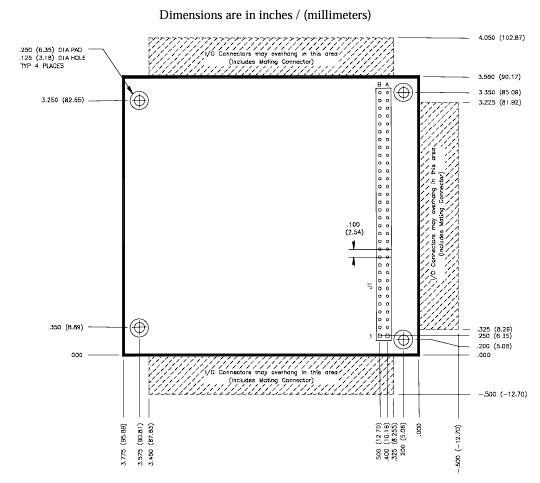
\includegraphics[width=0.7\linewidth]{imagenes/dim_pc104}
			\caption[Dimensiones del modulo para bus de 8 bits (Fuente: PC-104 Specification)]{Dimensiones del modulo para bus de 8 bits (Fuente: PC-104 Specification)}
			\label{fig:dimpc104}
		\end{figure}\newpage
		
		\item Opciones de Apilamiento de Módulos:Cada uno de los dos tipos de bus (8 bits y 16 bits) ofrece dos opciones de bus, según si los conectores de bus P1 y P2 se extienden a través del módulo como conectores "stackthrough" (de apilamiento pasante). Estas opciones se proporcionan para ayudar a cumplir con los estrictos requisitos de espacio de las aplicaciones embebidas.
		
		\begin{figure}[h!]
			\centering
			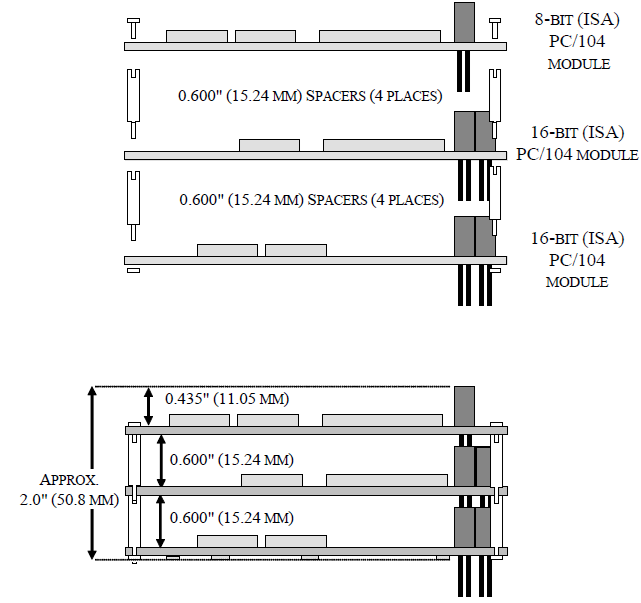
\includegraphics[width=0.8\linewidth]{imagenes/stack_pc104}
			\caption[Apilamientos de modulos de 8 y 16 bits (Fuente: PC-104 Specification)]{Apilamientos de modulos de 8 y 16 bits (Fuente: PC-104 Specification)}
			\label{fig:stackpc104}
		\end{figure}
		
		Nota: La figura  ilustra una pila de módulos típica que incluye módulos de 8 y 16 bits, y muestra el uso de las opciones de bus \textbf{stackthrough} y \textbf{non-stackthrough} (sin apilamiento pasante). Como se muestra en la figura , cuando se combinan módulos de 8 y 16 bits en una pila, los módulos de 16 bits deben apilarse debajo (es decir, en el "lado secundario") de los módulos de 8 bits. Opcionalmente, se puede incluir un conector de bus P2 "pasivo" en el diseño de los módulos de 8 bits, para permitir el uso de estos módulos en cualquier lugar de una pila.
		
		\item Ubicaciones de Clave (Key Locations): Se han designado ubicaciones de clave que consisten en pines omitidos en P1 y P2, y agujeros tapados en J1 y J2 en cada conector de bus, para ayudar a asegurar un acoplamiento correcto del conector.Como se muestra en (Cuadro 3º) los conectores B10 y C19
		
		\begin{table}[h!]
			\centering
			\label{tab:pc104_pinout}
			\small % Hace la fuente un poco más pequeña para que quepa mejor
			
			% --- Tabla para el conector J2/P2 (16-bit) ---
			\begin{minipage}{.48\textwidth}
				\centering
				\begin{tabular}{|c|l|l|}
					\hline % Línea horizontal superior
					\multicolumn{3}{|c|}{\textbf{J2/P2}} \\
					\hline % Línea horizontal debajo del título
					\textbf{Pin} & \textbf{Row D} & \textbf{Row C} \\
					\hline 
					0 & GND & GND \\
					\hline 
					1 & MEMCS16* & SBHE* \\
					\hline 
					2 & IOCS16* & LA23 \\
					\hline 
					3 & IRQ10 & LA22 \\
					\hline 
					4 & IRQ11 & LA21 \\
					\hline 
					5 & IRQ12 & LA20 \\
					\hline
					6 & IRQ15 & LA19 \\
					\hline 
					7 & IRQ14 & LA18 \\
					\hline 
					8 & DACK0* & LA17 \\
					\hline 
					9 & DRQ0 & MEMR* \\
					\hline 
					10 & DACK5* & MEMW* \\
					\hline 
					11 & DRQ5 & SD8 \\
					\hline 
					12 & DACK6* & SD9 \\
					\hline 
					13 & DRQ6 & SD10 \\
					\hline 
					14 & DACK7* & SD11 \\
					\hline 
					15 & DRQ7 & SD12 \\
					\hline 
					16 & +5V & SD13 \\
					\hline 
					17 & MASTER* & SD14 \\
					\hline 
					18 & GND & SD15 \\
					\hline 
					19 & GND & KEY \\
					\hline 
				\end{tabular}
			\end{minipage}
			\hfill % Espacio flexible entre las dos tablas
			% --- Tabla para el conector J1/P1 (8-bit) ---
			\begin{minipage}{.48\textwidth}
				\centering
				\begin{tabular}{|c|l|l|}
					\hline 
					\multicolumn{3}{|c|}{\textbf{J1/P1}} \\
					\hline 
					\textbf{Pin} & \textbf{Row A} & \textbf{Row B} \\
					\hline 
					1 & IOCHK* & GND \\
					\hline 
					2 & SD7 & RESET \\
					\hline 
					3 & SD6 & +5V \\
					\hline 
					4 & SD5 & IRQ9 \\
					\hline 
					5 & SD4 & -5V \\
					\hline 
					6 & SD3 & DRQ2 \\
					\hline 
					7 & SD2 & -12V \\
					\hline
					8 & SD1 & SRDY* \\
					\hline
					9 & SD0 & +12V \\
					\hline 
					10 & IOCHRDY & KEY \\
					\hline 
					11 & AEN & SMEMW* \\
					\hline 
					12 & SA19 & SMEMR* \\
					\hline 
					13 & SA18 & IOW* \\
					\hline
					14 & SA17 & IOR* \\
					\hline 
					15 & SA16 & DACK3* \\
					\hline
					16 & SA15 & DRQ3 \\
					\hline 
					17 & SA14 & DACK1* \\
					\hline 
					18 & SA13 & DRQ1 \\
					\hline 
					19 & SA12 & REFRESH* \\
					\hline 
					20 & SA11 & BCLK \\
					\hline 
					21 & SA10 & IRQ7 \\
					\hline 
					22 & SA9 & IRQ6 \\
					\hline
					23 & SA8 & IRQ5 \\
					\hline 
					24 & SA7 & IRQ4 \\
					\hline 
					25 & SA6 & IRQ3 \\
					\hline 
					26 & SA5 & DACK2* \\
					\hline 
					27 & SA4 & TC \\
					\hline
					28 & SA3 & BALE \\
					\hline 
					29 & SA2 & +5V \\
					\hline 
					30 & SA1 & OSC \\
					\hline 
					31 & SA0 & GND \\
					\hline 
					32 & GND & GND \\
					\hline 
				\end{tabular}
			\end{minipage}
			\caption{Asignaciones de Señales del Bus ISA de 8 y 16 bits}
		\end{table}
	\end{enumerate}
	
	\begin{figure}[h!]
		\centering
		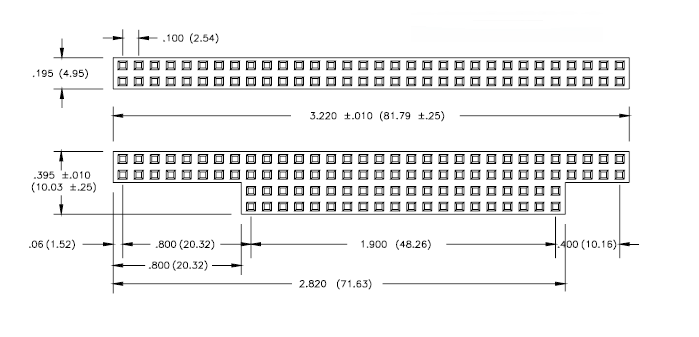
\includegraphics[width=0.7\linewidth]{imagenes/pin_pc104}
		\caption[Dimensiones de los conectores ISA para 8 y 16 bits (Fuente: PC-104 Specification)]{Dimensiones de los conectores ISA para 8 y 16 bits (Fuente: PC-104 Specification)}
		\label{fig:pinpc104}
	\end{figure}
	
	
	\newpage
	\subsubsection{Definición de señales ISA}
	La Industry Standard Architecture (ISA) \cite{Solari1992ISAandEISA} es un bus de expansión para computadoras que define la forma en que la CPU se comunica con dispositivos periféricos a través de líneas compartidas de dirección, datos y control. La Extended Industry Standard Architecture (EISA) es una extensión de este bus que amplía el ancho de datos a 32 bits, incorpora mayor capacidad de direccionamiento de memoria y añade soporte para configuración por software y arbitraje entre múltiples dispositivos, manteniendo compatibilidad con el estándar ISA.
	
	\subsubsection*{Direcciones y datos}
	\begin{enumerate}
		\item \textbf{BALE (Bus Address Latch Enable)}: La línea de Habilitación del Latch de Dirección del Bus es controlada por la CPU de la plataforma para indicar cuándo \texttt{SA<19:0>}, \texttt{LA<23:17>}, \texttt{AENx} y \texttt{SBHE*} son válidos. También se activa a un uno lógico cuando una tarjeta adicional ISA o un controlador DMA es dueño del bus.
		
		\item \textbf{SA<19:0> (Address lines)}: Las líneas de dirección son controladas por el maestro del bus ISA para definir las 20 líneas de señal de dirección inferiores necesarias para el primer 1 MB del espacio de direcciones de memoria.
		
		\item \textbf{LA<23:17> (Latched Address lines)}: Las líneas de Dirección Enclavadas (Latched) son controladas por el maestro del bus ISA o el controlador DMA para proporcionar las líneas de dirección adicionales requeridas para el espacio de direcciones de memoria de 16 MB.
		
		\item \textbf{SBHE* (System Byte High Enable)}: La línea de Habilitación de Byte Alto del Sistema es controlada por el maestro del bus ISA para indicar que hay datos válidos en las líneas \texttt{SD<15:8>}.
		
		\item \textbf{AENx (Address Enable)}: La línea de Habilitación de Dirección es controlada por la circuitería de la plataforma como una indicación a los recursos ISA para que no respondan a las líneas de DIRECCIÓN y COMANDO de E/S. Esta línea es el método por el cual se informa a los recursos de E/S que está ocurriendo un ciclo de transferencia DMA y que solo el recurso de E/S con una señal \texttt{DACKx*} activa puede responder a las líneas de señal de E/S.
		
		\item \textbf{SD<15:0> (Data lines)}: Las líneas de datos 0-7 u 8-15 se utilizan para un ciclo de 8 bits de datos, y las líneas 0-15 se utilizan para un ciclo de 16 bits de datos.
	\end{enumerate}
	
	\subsubsection*{Control de ciclo}
	\begin{enumerate}
		\item \textbf{MEMR* (Memory Read)}: La línea de Lectura de Memoria es controlada por el maestro del bus ISA o el controlador DMA para solicitar que un recurso de memoria coloque datos en el bus durante el ciclo.
		
		\item \textbf{SMEMR* (System Memory Read)}: La línea de Lectura de Memoria del Sistema se utiliza para solicitar que un recurso de memoria coloque datos en el bus durante el ciclo. Esta línea está activa cuando \texttt{MEMR*} está activa y las líneas \texttt{LA<23:20>} indican el primer 1 MB del espacio de direcciones.
		
		\item \textbf{MEMW* (Memory Write)}: La línea de Escritura de Memoria se utiliza para solicitar que un recurso de memoria acepte datos de las líneas de datos.
		
		\item \textbf{SMEMW* (System Memory Write)}: La línea de Escritura de Memoria del Sistema se utiliza para solicitar que un recurso de memoria coloque datos en el bus durante el ciclo. Esta línea está activa cuando \texttt{MEMW\#} está activa y las líneas \texttt{LA<23:20>} indican el primer 1 MB.
		
		\item \textbf{IOR* (I/O Read)}: La línea de Lectura de E/S es controlada por el maestro del bus ISA o el controlador DMA para solicitar que un recurso de E/S coloque datos en el bus de datos durante el ciclo.
		
		\item \textbf{IOW* (I/O Write)}: La Escritura de E/S solicita que un recurso de E/S acepte datos del bus de datos.
		
		\item \textbf{MEMCS16* (Memory Chip Select 16)}: La línea de Selección de Chip de Memoria 16 es controlada por el recurso de memoria para indicar que es un recurso ISA que soporta un ciclo de acceso de 16 bits de datos.
		
		\item \textbf{IOCS16* (I/O Chip Select 16)}: La línea de Selección de Chip de E/S 16 es controlada por un recurso de E/S para indicar que es un recurso ISA que soporta un ciclo de acceso de 16 bits de datos.
		
		\item \textbf{IOCHRDY (I/O Channel Ready)}: La línea de Canal de E/S Listo permite a los recursos indicar al maestro del bus ISA que se requiere tiempo de ciclo adicional.
		
		\item \textbf{SRDY* (Synchronous Ready)}: La línea de Listo Síncrono (o NOWS* No-Wait-State) es activada por el recurso accedido para indicar que se puede ejecutar un ciclo de acceso más corto que el estándar.
	\end{enumerate}
	
	\subsubsection*{Control del Bus}
	\begin{enumerate}
		\item \textbf{REFRESH* (Memory Refresh)}: Es controlada por el controlador de refresco para indicar un ciclo de refresco.
		
		\item \textbf{MASTER16*}: La línea \texttt{MASTER16\#} solo es activada por una tarjeta propietaria del bus adicional ISA a la que el controlador DMA le ha concedido la propiedad del bus.
		
		\item \textbf{IOCHK* (I/O Channel Check)}: La línea de Verificación de Canal de E/S es controlada por cualquier recurso. Se activa para una condición de error general que no tiene una interpretación específica.
		
		\item \textbf{RESET}: La línea de Reset es activada por la circuitería de la plataforma. Cualquier recurso del bus que detecte una señal de RESET activa debe poner inmediatamente en alta impedancia (tri-state) todos sus controladores de salida.
		
		\item \textbf{BCLK (System Bus Clock)}: La línea de Reloj del Bus del Sistema es un reloj controlado por la circuitería de la plataforma. Tiene un ciclo de trabajo del 50\% $\pm$ 5\% (57 a 69 ns para 8 MHz), a una frecuencia de 6 a 8 MHz.
		
		\item \textbf{OSC (Oscillator)}: La línea del Oscilador es un reloj controlado por la circuitería de la plataforma. Tiene un ciclo de trabajo del 45-55\%, a una frecuencia de 14.31818 MHz. No está sincronizado con ninguna otra señal del bus.
	\end{enumerate}
	
	\subsubsection*{Interrupción}
	\begin{enumerate}
		\item \textbf{IRQX (Interrupt Request)}: Las líneas de Petición de Interrupción permiten a las tarjetas adicionales solicitar servicio de interrupción por parte de la CPU de la plataforma.
	\end{enumerate}
	
	\subsubsection*{DMA}
	\begin{enumerate}
		\item \textbf{DRQX (DMA Request)}: Las líneas de Petición de DMA son activadas por los recursos de E/S para solicitar servicio por parte del controlador DMA de la plataforma.
		
		\item \textbf{DACKX* (DMA Acknowledge)}: Las líneas de Reconocimiento de DMA son activadas por el controlador DMA de la plataforma para seleccionar el recurso de E/S que solicitó un ciclo de transferencia DMA.
		
		\item \textbf{TC (Terminal Count)}: La línea de Conteo Terminal es controlada por el controlador DMA de la plataforma para indicar que todos los datos han sido transferidos.
	\end{enumerate}
	
	\subsubsection{Especificaciones eléctricas}
	\begin{enumerate}
		\item Asignación de señales: Las señales se asignan en el mismo orden que en los conectores de borde de tarjeta del bus ISA, pero se transforman a los pines correspondientes del conector de cabezal (header).
		
		\item Tierras adicionales: Se han añadido varios pines de tierra para maximizar la integridad del bus.
		
		\item Temporización de Señales de CA (AC): Todas las señales del bus PC/104 son idénticas en su temporización a sus contrapartes del bus ISA.
		
		\item Niveles de Señales de CC (DC): Todos los niveles de voltaje de lógica alta y lógica baja de las señales del bus PC/104 son idénticos a sus contrapartes del bus ISA
		
		\item Corriente de Excitación del Bus (Bus Drive Current): Para reducir el número de componentes y minimizar el consumo de energía y la disipación de calor, la mayoría de las señales del bus tienen un requisito de corriente de excitación reducido a 4 mA. La excepción son las señales de colector abierto, que deben poder manejar las resistencias de pull-up de 330 ohmios definidas por la especificación ISA. Esto permite el control directo del bus por parte de muchos dispositivos ASIC y por lógica de la familia HCT. Específicamente, las siguientes señales deben ser controladas con dispositivos capaces de proporcionar 20 mA de corriente de sumidero (sink current), como se indica en la especificación ISA:
			\subitem  $\bullet$ \textbf{MEMCS16* (Memory Chip Select 16)}
			\subitem  $\bullet$ \textbf{IOCS16* (I/O Chip Select 16)}
			\subitem  $\bullet$ \textbf{MASTER16*}
			\subitem  $\bullet$ \textbf{SRDY* (Synchronous Ready)}\newline
			
		Todas las demás señales pueden ser controladas con dispositivos capaces de proporcionar 4 mA de corriente de sumidero
		
		\item  Opción de Interrupción Compartida: Existe un método opcional para compartir una única línea de interrupción del bus entre múltiples dispositivos. El apéndice  proporciona una guía de diseño que puede ayudar a asegurar la compatibilidad de esta función entre módulos PC/104.
		
		\item Opción de Terminación del Bus: En algunos sistemas puede ser deseable la terminación de las señales del bus ISA de 8 y 16 bits para aumentar la integridad de los datos y la fiabilidad del sistema. Cuando se incluye la terminación, se deben utilizar redes de terminación de CA para proporcionar una terminación cercana a la impedancia característica de las líneas de señal, sin exceder las capacidades de corriente de salida de CC de los controladores.
		
		\item Requisitos de Alimentación del Módulo: El rango de voltaje operativo y los requisitos máximos de potencia de cada módulo se indican en la siguiente tabla. Cada módulo no debe consumir más de la corriente de funcionamiento indicada. La potencia total requerida por una pila de módulos PC/104 es la suma de la requerida por cada uno de los módulos en la pila. Los voltajes operativos, que se miden en los pines del conector del bus de cualquier módulo, se especifican con una tolerancia de ±5\%
		
		\begin{table}[h!]
			\centering
			
			\label{tab:power_requirements}
			\begin{tabular}{|l|c|c|c|}
				\hline
				\textbf{Voltaje Nominal} & \textbf{Voltaje Máximo} & \textbf{Voltaje Mínimo} & \textbf{Corriente Máxima} \\
				\hline
				+12 Volts & +12.6 Volts & +11.4 Volts & 1.0 Amp \\
				\hline
				+5 Volts  & +5.25 Volts & +4.75 Volts & 2.0 Amp \\
				\hline
				-5 Volts  & -4.75 Volts & -5.25 Volts & 0.2 Amp \\
				\hline
				-12 Volts & -11.4 Volts & -12.6 Volts & 0.3 Amp \\
				\hline
			\end{tabular}
			\caption{Requisitos de Alimentación del Módulo}
		\end{table}
	\end{enumerate}
	
	\subsubsection{Niveles de conformidad}
	Esta sección proporciona la terminología destinada a ayudar a los fabricantes y usuarios de productos compatibles con PC1-04 a definir y especificar la conformidad de las especificaciones PC-104
	\begin{enumerate}
		\item PC-104 Compatible: Esto refiere a los dispositivos con factor de forma PC-104 que cumplen con todos los aspectos no opcionales de la especificación PC-104, incluidas las mecánicas y eléctricas.
		
		\item PC-104 Compatible con el bus: Refiere a los dispositivos que no tienen el factor de forma PC-104 (es decir que no cumplen con sus dimensiones del modulo), pero proporcionan un conector de bus PC-104 macho o hembra que cumplen con las especificaciones mecánicas y eléctricas proporcionadas por el estándar.
	\end{enumerate}
	
	\subsection{Estandar PC-104 plus}
	A medida que avanzaron los requisitos tecnológicos, comenzó a surgir la necesidad de un mayor rendimiento de la velocidad de transferencia del bus. Esto es especialmente cierto en lo que respecta a los dispositivos gráficos, así como a otros dispositivos de E/S de alta velocidad, como las redes. El Consorcio PC/104 afrontó este desafío incorporando un bus PCI en el formato PC/104, que pasó a ser conocido como PC/104-Plus. Esta arquitectura proporciona un enlace a hardware heredado versátil mientras satisface los requisitos de alta velocidad para el hardware presente y futuro. El documento \cite{pc104plus:spec2008_report} suministra las especificaciones mecánicas y eléctricas para el \textbf{PC/104-Plus} e incorpora todas las características del PC/104, con la ventaja añadida del bus PCI de alta velocidad. El tamaño físico, la configuración de montaje y la porción de interconexión eléctrica de la especificación PC/104 permanecerán sin cambios.Las principales diferencias entre PC/104 y PC/104-plus son:
	
	\begin{enumerate}
		\item Un tercer conector opuesto a los conectores ISA es compatible con el bus PCI.
		
		\item La altura de los componentes en la cara superior se ha reducido de 0.435$"$ a 0.345$"$ y la inferior se ha incrementado de 0.100$"$ a 0.190$"$ para aumentar la flexibilidad del módulo.
		
		\item Se ha añadido lógica de control para manejar los requisitos del bus de alta velocidad.
	\end{enumerate}
	
	\begin{figure}
		\centering
		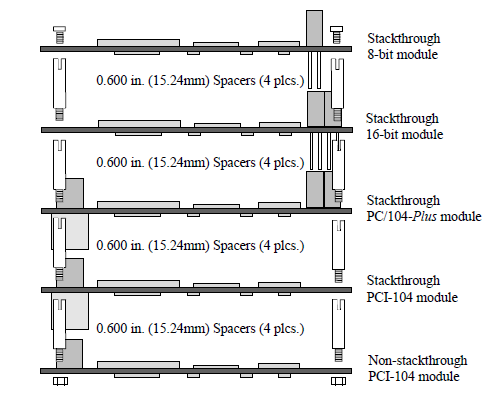
\includegraphics[width=0.7\linewidth]{imagenes/stack_pc104_p}
		\caption[Posibles configuraciones de apilamiento (Fuente:PC/104-Plus Specification Version 2.3)]{Posibles configuraciones de apilamiento (Fuente:PC/104-Plus Specification Version 2.3)}
		\label{fig:stackpc104p}
	\end{figure}
	
	\subsubsection{Especificaciones mecánicas}
	\begin{enumerate}
		\item Las especificaciones mecánicas para el bus ISA se definen en la Especificación PC/104. El conector y su colocación en el PC/104-Plus se muestran en las siguientes figuras:
		\begin{figure}[h!]
			\centering
			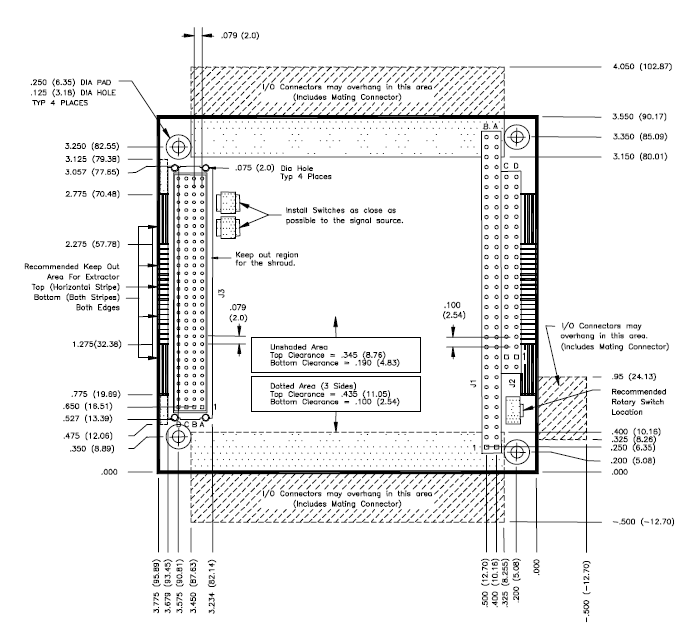
\includegraphics[width=0.7\linewidth]{imagenes/mec_pc104p}
			\caption[Colocación PCI estándar PC/104-plus]{Colocación PCI estándar PC/104-plus (Fuente:PC/104-Plus Specification Version 2.3)}
			\label{fig:mecpc104p}
		\end{figure}
		
		\item Los relojes están ajustados en el Host Board de tal manera que la longitud de la pista CLK3 es 0.662$"$ menor que CLK2, la pista CLK2 es 0.662$"$ menor que CLK1, y la pista CLK1 es 0.662$"$ menor que CLK0. Por lo tanto, el primer módulo de la pila debe seleccionar CLK0 (la pista más larga), el segundo CLK1, etc. Esto proporciona casi ninguna desviación de sincronización (skew) entre módulos. Las longitudes de pista están indicadas en la Revisión 2.2 \cite{pci:spec1998_report} de la Especificación del Bus Local PCI.
		
		\item Las dimensiones mecánicas para este módulo son idénticas a la Especificación PC/104.
		
		\item El conector para el bus PCI es un conector de paso de 2 mm 4×30 (120 pines). La cubierta (shroud) debe instalarse en la parte inferior de la tarjeta PCI cuando se utiliza un conector stack-through (apilable).
		
		\item Los fabricantes de módulos PC/104-Plus deben etiquetar claramente cerca o en el conector PCI la capacidad de señalización PCI del módulo. La etiqueta es para garantizar la correcta instalación del módulo. Dependiendo del tipo de tarjeta, la etiqueta será una de las siguientes:
		\begin{itemize}
			\item Solo 3.3V
			
			\item Solo 5V
			
			\item Universal 
		\end{itemize}
	\end{enumerate}
	
	
	\subsubsection{Definición de señales del bus PCI}
	La siguiente figura muestra los pines en grupos funcionales, con los pines requeridos a la izquierda y los pines opcionales a la derecha. Los pines sombreados a la derecha son características no soportadas, pero se incluyen para mostrar el bus PCI completo tal como se define en la Revisión 2.2 de la Especificación del Bus Local PCI. Esta versión del bus PCI está diseñada para ser un bus de 32 bits que funciona a 33 MHz y, por lo tanto, la extensión de 64 bits y 66 MHz no son compatibles en este momento. Tampoco son compatibles las características de boundary scan (JTAG), la de presencia (Present), y la de reloj en funcionamiento (Clock running). La indicación de dirección en los pines asume un dispositivo maestro/destino combinado.
	
	\begin{figure}
		\centering
		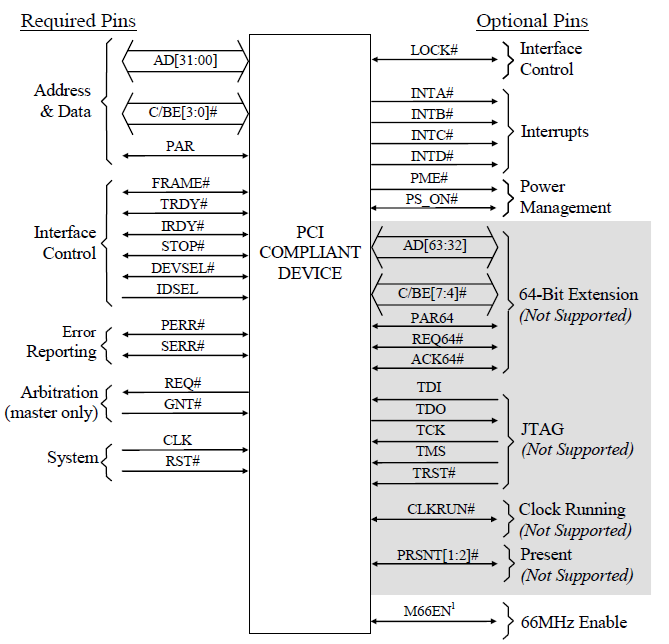
\includegraphics[width=1\linewidth]{imagenes/signlas_pc104p}
		\caption[Definición de señales para el bus (Fuente:PC/104-Plus Specification Version 2.3)]{Definición  de señales para el bus (Fuente:PC/104-Plus Specification Version 2.3)}
		\label{fig:signlaspc104p}
	\end{figure}
	
	\subsubsection*{Dirección y Datos}
	\begin{enumerate}
		\item \textbf{AD[31:00] (Address and Data)}: La \textbf{Dirección y los Datos} se \textbf{multiplexan} en los mismos pines PCI. Una transacción de bus consiste en una fase de dirección seguida por una o más fases de datos.
		
		\item \textbf{C/BE[3:0]\# (Bus Command/Byte Enables)}: Los \textbf{Comandos de Bus/Habilitadores de Byte} se multiplexan. Durante la fase de dirección de una transacción, definen el comando de bus. Durante la fase de datos, se usan como habilitadores de byte.
		
		\item \textbf{PAR (Parity)}: La \textbf{Paridad} es par a través de AD[31:00] y C/BE[3:0]\#. La generación de paridad es requerida por todas las señales PCI.
	\end{enumerate}
	
	\subsubsection*{Pines de Control de Interfaz}
	\begin{enumerate}
		\item \textbf{FRAME\# (Cycle Frame)}: Marco de Ciclo es conducido por el maestro actual para indicar el comienzo de un acceso y permanecerá activo hasta el ciclo de datos final.
		
		\item \textbf{TRDY\# (Target Ready)}: Destino Listo indica la capacidad del dispositivo seleccionado para completar la fase de datos actual de la transacción. Tanto \textbf{IRDY\#} como \textbf{TRDY\#} deben estar afirmados para terminar un ciclo de datos.
		
		\item \textbf{IRDY\# (Initiator Ready)}: Iniciador Listo indica la capacidad del maestro del bus para completar la fase de datos actual de la transacción.
		
		\item \textbf{STOP\# (Stop)}: Parada indica que el dispositivo actualmente seleccionado está solicitando al maestro que detenga la transacción actual.
		
		\item \textbf{DEVSEL\# (Device Select)}: Selección de Dispositivo, cuando es conducida activamente, indica que el dispositivo conductor ha decodificado su dirección como el objetivo del acceso actual.
		
		\item \textbf{IDSEL (Initialization Device Select)}: Selección de Dispositivo de Inicialización se utiliza como un *chip-select* (selección de chip) durante las transacciones de lectura y escritura de configuración.
		
		\item \textbf{LOCK\# (Lock)}: Bloqueo indica una operación atómica a un puente (*bridge*) que puede requerir múltiples transacciones para completarse.
	\end{enumerate}
	
	\subsubsection*{Reporte de Errores}
	\begin{enumerate}
		\item \textbf{PERR\# (Parity Error)}: Error de Paridad se utiliza para reportar errores de paridad de datos.
		
		\item \textbf{SERR\# (System Error)}: Error de Sistema se utiliza para reportar errores de paridad de dirección.
	\end{enumerate}
	
	\subsubsection*{Arbitraje (Solo Maestros de Bus)}
	\begin{enumerate}
		\item \textbf{REQ\# (Request)}: Solicitud indica al árbitro que este dispositivo desea usar el bus.
		
		\item \textbf{GNT\# (Grant)}: Concesión indica al dispositivo solicitante que se le ha otorgado el acceso.
	\end{enumerate}
	
	\subsubsection*{Sistema}
	\begin{enumerate}
		\item \textbf{CLK (Clock)}: Reloj proporciona la temporización para todas las transacciones en el bus PCI y es una entrada para cada dispositivo PCI.
		
		\item \textbf{RST\# (Reset)}: Reinicio se utiliza para llevar los registros, secuenciadores y señales específicos de PCI a un estado consistente.
		
		\item \textbf{M66EN (66 MHz Enable)}: Habilitación de 66 MHz indica a un dispositivo si el segmento de bus está operando a 33 MHz o 66 MHz. El bus PCI ha sido simulado a 33 MHz. Para el propósito de esta especificación, \textbf{66 MHz no es soportado}. Para soportar futuras mejoras, la señal \textbf{M66EN} debe estar conectada a tierra (*grounded*) en cualquier módulo que no soporte 66 MHz y dejarse abierta para módulos que puedan soportar un reloj de 66 MHz.
	\end{enumerate}
	
	\subsubsection*{Interrupciones}
	\begin{enumerate}
		\item \textbf{INTA\# (Interrupt A)}: Interrupción A se utiliza para solicitar Interrupciones.
		
		\item \textbf{INTB\# (Interrupt B)}: Interrupción B se utiliza para solicitar Interrupciones.
		
		\item \textbf{INTC\# (Interrupt C)}: Interrupción C se utiliza para solicitar Interrupciones.
		
		\item \textbf{INTD\# (Interrupt D)}: Interrupción D se utiliza para solicitar Interrupciones.
	\end{enumerate}
	
	\subsubsection*{Gestión de Energía}
	\begin{enumerate}
		\item \textbf{PME\# (Power Management Event)}: Evento de Gestión de Energía se utiliza para sacar a la CPU de estados de baja energía, como el *wake-on-LAN*.
		
		\item \textbf{PSON\# (Power Supply On)}: Encendido de la Fuente de Alimentación es una señal de control de suministro de energía que puede encender o apagar el suministro de energía.
		
		\item \textbf{+5V\_SB (+5 Volt Standby)}: \textbf{+5 Voltios en Espera} es una fuente de energía que siempre está presente cuando la energía principal es suministrada al sistema.
	\end{enumerate}
	
	\subsubsection*{Agrupamiento de señales}
	La arquitectura PC/104-Plus fue desarrollada para aprovechar la versatilidad y simplicidad del mercado de PC para las aplicaciones embebidas. Al igual que el PC de escritorio, PC/104-Plus tiene la capacidad de añadir tarjetas auxiliares para expandir las capacidades de la CPU. Pero en lugar de utilizar tarjetas de ranura (slot cards), PC/104-Plus añade módulos adicionales utilizando conectores apilables (stack-through connectors). Esto tiene dos ventajas: reduce el tamaño del sistema y hace que el sistema sea más robusto para que pueda resistir mejor los golpes y las vibraciones.Para lograr una arquitectura apilable (stack-through), se debe establecer un medio para seleccionar las señales apropiadas para cada tarjeta de expansión que permita fácilmente la instalación y configuración de los módulos PC/104-Plus y PCI-104. Las señales en cuestión incluyen las líneas CLKx, IDSELx, REQx, GNTx y INTx. Los ordenadores de escritorio normales superan este problema enrutando solo las señales necesarias a cada uno de los conectores de ranura. Por ejemplo, en un PC de escritorio, solo CLK1, IDSEL1, REQ1 y GNT1 se enrutan a la ranura PCI1. Del mismo modo, CLK2, IDSEL2, REQ2 y GNT2 se enrutan a la ranura 2.
	
	Las interrupciones en un PC de escritorio se manejan de una manera diferente. Las cuatro interrupciones del controlador de interrupciones se enrutan a cada conector de ranura PCI. Por convención, INTA en una tarjeta de expansión se utiliza para dispositivos de función única y las interrupciones restantes se utilizan en el caso de dispositivos multifuncionales. Esto podría suponer una gran carga para INTA, ya que todas las tarjetas de expansión utilizarían esta interrupción. Para aliviar la carga, los fabricantes de PC alternan las interrupciones en la placa base a cada uno de los conectores PCI. Esto se muestra en la figura 14 y 15.
	
	\begin{figure}[h!]
		\centering
		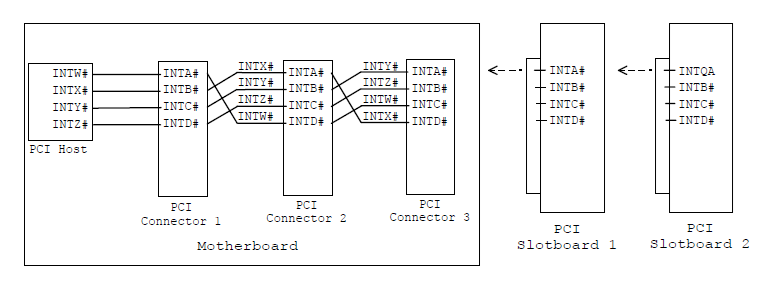
\includegraphics[width=1\linewidth]{imagenes/pci_pc104p}
		\caption[Ruteo de interrupciones para PC de escritorio]{Ruteo de interrupciones para PC de escritorio (Fuente:PC/104-Plus Specification Version 2.3)}
		\label{fig:pcipc104p}
	\end{figure}
	
	Dado que PC/104-Plus es una arquitectura apilable (stack-through), solo hay un conector al que deben conectarse todas las tarjetas de expansión. Se debe establecer un medio para seleccionar las señales apropiadas que permita fácilmente la instalación y configuración de los módulos adicionales PC/104-Plus y PCI-104. La figura  muestra un método que se puede aplicar a las tarjetas de expansión.\newpage
	
	\begin{figure}[h!]
		\centering
		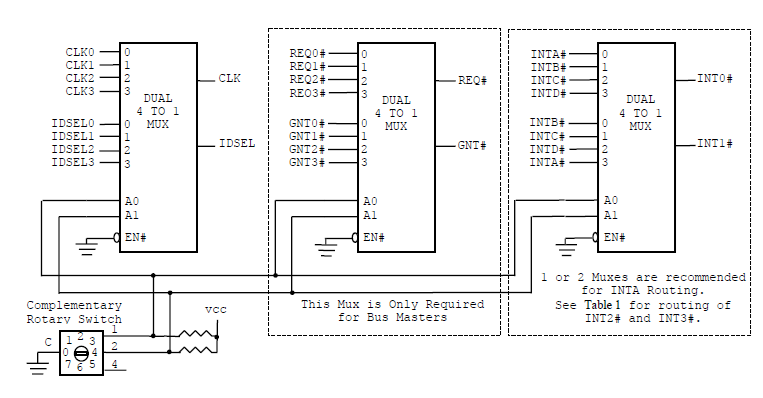
\includegraphics[width=1\linewidth]{imagenes/pci2_pc104p}
		\caption[Selección de señales en una placa de expansión]{Selección de señales en una placa de expansión (Fuente:PC/104-Plus Specification Version 2.3)}
		\label{fig:pci2pc104p}
	\end{figure}
	
	Los chips multiplexores en la tarjeta de expansión sirven como el equivalente a tener múltiples conectores de ranura PCI en la placa base de un PC de escritorio. Para seleccionar las señales apropiadas REQ, GNT, CLK e INT para el módulo de expansión, el interruptor rotatorio debe ajustarse a la posición en la pila. Para los módulos de expansión que requieren más de una interrupción, la alternancia (staggering) de las líneas INTx se logra en el módulo de expansión mediante el uso de multiplexores. La figura 16  muestra el enrutamiento de la interrupción en un Módulo Host PCI y en un módulo de expansión con dos funciones. La porción de Módulo Adicional de la figura muestra cómo el multiplexor de la derecha de la figura anterior encaja en un módulo adicional. Si una tarjeta tiene una función única, solo se requiere la mitad del multiplexor.
	
	\begin{figure}[h!]
		\centering
		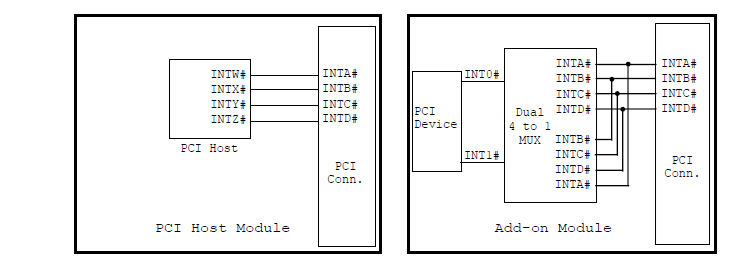
\includegraphics[width=1\linewidth]{imagenes/pci3_pc104p}
		\caption[Ruteo de INT (Fuente:PC/104-Plus Specification Version 2.3)]{Ruteo de INT (Fuente:PC/104-Plus Specification Version 2.3)}
		\label{fig:pci3pc104p}
	\end{figure}
	
	Los chips multiplexores son chips dual 4:1 Mux/Demux. Proporcionan un interruptor de 5 ohm que conecta la entrada y la salida juntas. Estos interruptores proporcionan una ruta bidireccional con un retraso de propagación de señal no mayor que el retraso RC de la resistencia de encendido del interruptor y la capacitancia de carga. Esto es típicamente 250ps con una carga de 50pF. Use un mux para 1 o 2 interrupciones o dos muxes para 3 o 4 . Aunque son posibles y permisibles otros métodos para configurar los módulos, el interruptor rotatorio es limpio y proporciona la menor probabilidad de error en la configuración.
	
	\begin{table}[h!]
		\centering
		\caption{\textbf{Configuraciones del Interruptor Rotatorio}}
		\label{tab:rotary_switch_settings}
		\small 
		\begin{tabular}{|c|c|c|c|c|c|c|c|c|}
			\hline
			\textbf{Posición del Interruptor} & \textbf{Módulo Slot} & \textbf{REQ\#} & \textbf{GNT\#} & \textbf{CLK} & \textbf{INT0\#} & \textbf{INT1\#} & \textbf{INT2\#} & \textbf{INT3\#} \\
			\hline
			0 o 4 & 1 & REQ0\# & GNT0\# & CLK0 & INTA\# & INTB\# & INTC\# & INTD\# \\
			\hline
			1 o 5 & 2 & REQ1\# & GNT1\# & CLK1 & INTB\# & INTC\# & INTD\# & INTA\# \\
			\hline
			2 o 6 & 3 & REQ2\# & GNT2\# & CLK2 & INTC\# & INTD\# & INTA\# & INTB\# \\
			\hline
			3 o 7 & 4 & REQ3\# & GNT3\# & CLK3 & INTD\# & INTA\# & INTB\# & INTC\# \\
			\hline
		\end{tabular}
	\end{table}
	
	\subsubsection*{3.3 +5V\_SB PSON y PME}
		Para soportar las fuentes de alimentación ATX y las funciones de apagado (power down) se han añadido tres señales al bus PCI. Estas son: +5V\_SB, que es una fuente de alimentación que siempre está presente cuando la energía principal se suministra al sistema; PSON, que es una señal de control de la fuente de alimentación que puede encender o apagar la fuente de alimentación; y PME, que puede utilizarse para sacar a la CPU de estados de apagado (power down states) como el wake-on-LAN.Estas señales se han implementado en los pines reservados del bus de expansión PCI de las especificaciones PC/104-Plus y PCI-104 en los pines B1, C9 y D10. No todos los fabricantes implementarán estas señales; por lo tanto, para mantener la compatibilidad con los productos existentes, es importante que los diseños que implementen estas funciones se protejan contra entradas no controladas (undriven inputs).
	
	
	
	
	
	\newpage
	\section{Conclusión}
	
	
	\newpage
	\section{Bibliografía}
	\printbibliography
	
	
\end{document}
